\documentclass[1p]{elsarticle_modified}
%\bibliographystyle{elsarticle-num}

%\usepackage[colorlinks]{hyperref}
%\usepackage{abbrmath_seonhwa} %\Abb, \Ascr, \Acal ,\Abf, \Afrak
\usepackage{amsfonts}
\usepackage{amssymb}
\usepackage{amsmath}
\usepackage{amsthm}
\usepackage{scalefnt}
\usepackage{amsbsy}
\usepackage{kotex}
\usepackage{caption}
\usepackage{subfig}
\usepackage{color}
\usepackage{graphicx}
\usepackage{xcolor} %% white, black, red, green, blue, cyan, magenta, yellow
\usepackage{float}
\usepackage{setspace}
\usepackage{hyperref}

\usepackage{tikz}
\usetikzlibrary{arrows}

\usepackage{multirow}
\usepackage{array} % fixed length table
\usepackage{hhline}

%%%%%%%%%%%%%%%%%%%%%
\makeatletter
\renewcommand*\env@matrix[1][\arraystretch]{%
	\edef\arraystretch{#1}%
	\hskip -\arraycolsep
	\let\@ifnextchar\new@ifnextchar
	\array{*\c@MaxMatrixCols c}}
\makeatother %https://tex.stackexchange.com/questions/14071/how-can-i-increase-the-line-spacing-in-a-matrix
%%%%%%%%%%%%%%%

\usepackage[normalem]{ulem}

\newcommand{\msout}[1]{\ifmmode\text{\sout{\ensuremath{#1}}}\else\sout{#1}\fi}
%SOURCE: \msout is \stkout macro in https://tex.stackexchange.com/questions/20609/strikeout-in-math-mode

\newcommand{\cancel}[1]{
	\ifmmode
	{\color{red}\msout{#1}}
	\else
	{\color{red}\sout{#1}}
	\fi
}

\newcommand{\add}[1]{
	{\color{blue}\uwave{#1}}
}

\newcommand{\replace}[2]{
	\ifmmode
	{\color{red}\msout{#1}}{\color{blue}\uwave{#2}}
	\else
	{\color{red}\sout{#1}}{\color{blue}\uwave{#2}}
	\fi
}

\newcommand{\Sol}{\mathcal{S}} %segment
\newcommand{\D}{D} %diagram
\newcommand{\A}{\mathcal{A}} %arc


%%%%%%%%%%%%%%%%%%%%%%%%%%%%%5 test

\def\sl{\operatorname{\textup{SL}}(2,\Cbb)}
\def\psl{\operatorname{\textup{PSL}}(2,\Cbb)}
\def\quan{\mkern 1mu \triangleright \mkern 1mu}

\theoremstyle{definition}
\newtheorem{thm}{Theorem}[section]
\newtheorem{prop}[thm]{Proposition}
\newtheorem{lem}[thm]{Lemma}
\newtheorem{ques}[thm]{Question}
\newtheorem{cor}[thm]{Corollary}
\newtheorem{defn}[thm]{Definition}
\newtheorem{exam}[thm]{Example}
\newtheorem{rmk}[thm]{Remark}
\newtheorem{alg}[thm]{Algorithm}

\newcommand{\I}{\sqrt{-1}}
\begin{document}

%\begin{frontmatter}
%
%\title{Boundary parabolic representations of knots up to 8 crossings}
%
%%% Group authors per affiliation:
%\author{Yunhi Cho} 
%\address{Department of Mathematics, University of Seoul, Seoul, Korea}
%\ead{yhcho@uos.ac.kr}
%
%
%\author{Seonhwa Kim} %\fnref{s_kim}}
%\address{Center for Geometry and Physics, Institute for Basic Science, Pohang, 37673, Korea}
%\ead{ryeona17@ibs.re.kr}
%
%\author{Hyuk Kim}
%\address{Department of Mathematical Sciences, Seoul National University, Seoul 08826, Korea}
%\ead{hyukkim@snu.ac.kr}
%
%\author{Seokbeom Yoon}
%\address{Department of Mathematical Sciences, Seoul National University, Seoul, 08826,  Korea}
%\ead{sbyoon15@snu.ac.kr}
%
%\begin{abstract}
%We find all boundary parabolic representation of knots up to 8 crossings.
%
%\end{abstract}
%\begin{keyword}
%    \MSC[2010] 57M25 
%\end{keyword}
%
%\end{frontmatter}

%\linenumbers
%\tableofcontents
%
\newcommand\colored[1]{\textcolor{white}{\rule[-0.35ex]{0.8em}{1.4ex}}\kern-0.8em\color{red} #1}%
%\newcommand\colored[1]{\textcolor{white}{ #1}\kern-2.17ex	\textcolor{white}{ #1}\kern-1.81ex	\textcolor{white}{ #1}\kern-2.15ex\color{red}#1	}

{\Large $\underline{12a_{0463}~(K12a_{0463})}$}

\setlength{\tabcolsep}{10pt}
\renewcommand{\arraystretch}{1.6}
\vspace{1cm}\begin{tabular}{m{100pt}>{\centering\arraybackslash}m{274pt}}
\multirow{5}{120pt}{
	\centering
	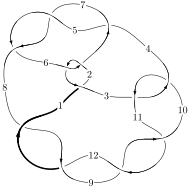
\includegraphics[width=112pt]{../../../GIT/diagram.site/Diagrams/png/1264_12a_0463.png}\\
\ \ \ A knot diagram\footnotemark}&
\allowdisplaybreaks
\textbf{Linearized knot diagam} \\
\cline{2-2}
 &
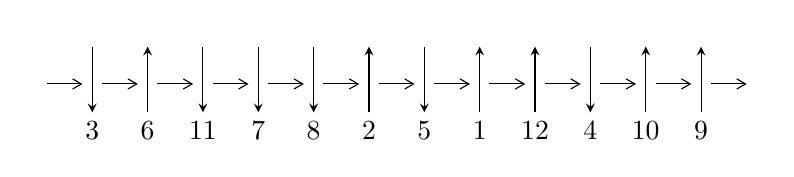
\begin{tikzpicture}[x=20pt, y=17pt]
	% nodes
	\node (C0) at (0, 0) {};
	\node (C1) at (1, 0) {};
	\node (C1U) at (1, +1) {};
	\node (C1D) at (1, -1) {3};

	\node (C2) at (2, 0) {};
	\node (C2U) at (2, +1) {};
	\node (C2D) at (2, -1) {6};

	\node (C3) at (3, 0) {};
	\node (C3U) at (3, +1) {};
	\node (C3D) at (3, -1) {11};

	\node (C4) at (4, 0) {};
	\node (C4U) at (4, +1) {};
	\node (C4D) at (4, -1) {7};

	\node (C5) at (5, 0) {};
	\node (C5U) at (5, +1) {};
	\node (C5D) at (5, -1) {8};

	\node (C6) at (6, 0) {};
	\node (C6U) at (6, +1) {};
	\node (C6D) at (6, -1) {2};

	\node (C7) at (7, 0) {};
	\node (C7U) at (7, +1) {};
	\node (C7D) at (7, -1) {5};

	\node (C8) at (8, 0) {};
	\node (C8U) at (8, +1) {};
	\node (C8D) at (8, -1) {1};

	\node (C9) at (9, 0) {};
	\node (C9U) at (9, +1) {};
	\node (C9D) at (9, -1) {12};

	\node (C10) at (10, 0) {};
	\node (C10U) at (10, +1) {};
	\node (C10D) at (10, -1) {4};

	\node (C11) at (11, 0) {};
	\node (C11U) at (11, +1) {};
	\node (C11D) at (11, -1) {10};

	\node (C12) at (12, 0) {};
	\node (C12U) at (12, +1) {};
	\node (C12D) at (12, -1) {9};
	\node (C13) at (13, 0) {};

	% arrows
	\draw[->,>={angle 60}]
	(C0) edge (C1) (C1) edge (C2) (C2) edge (C3) (C3) edge (C4) (C4) edge (C5) (C5) edge (C6) (C6) edge (C7) (C7) edge (C8) (C8) edge (C9) (C9) edge (C10) (C10) edge (C11) (C11) edge (C12) (C12) edge (C13) ;	\draw[->,>=stealth]
	(C1U) edge (C1D) (C2D) edge (C2U) (C3U) edge (C3D) (C4U) edge (C4D) (C5U) edge (C5D) (C6D) edge (C6U) (C7U) edge (C7D) (C8D) edge (C8U) (C9D) edge (C9U) (C10U) edge (C10D) (C11D) edge (C11U) (C12D) edge (C12U) ;
	\end{tikzpicture} \\
\hhline{~~} \\& 
\textbf{Solving Sequence} \\ \cline{2-2} 
 &
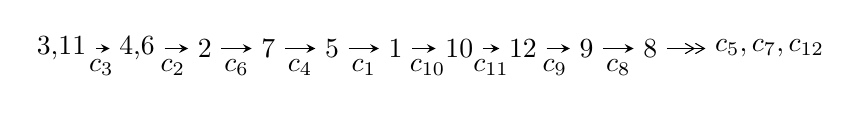
\begin{tikzpicture}[x=23pt, y=7pt]
	% node
	\node (A0) at (-1/8, 0) {3,11};
	\node (A1) at (17/16, 0) {4,6};
	\node (A2) at (17/8, 0) {2};
	\node (A3) at (25/8, 0) {7};
	\node (A4) at (33/8, 0) {5};
	\node (A5) at (41/8, 0) {1};
	\node (A6) at (49/8, 0) {10};
	\node (A7) at (57/8, 0) {12};
	\node (A8) at (65/8, 0) {9};
	\node (A9) at (73/8, 0) {8};
	\node (C1) at (1/2, -1) {$c_{3}$};
	\node (C2) at (13/8, -1) {$c_{2}$};
	\node (C3) at (21/8, -1) {$c_{6}$};
	\node (C4) at (29/8, -1) {$c_{4}$};
	\node (C5) at (37/8, -1) {$c_{1}$};
	\node (C6) at (45/8, -1) {$c_{10}$};
	\node (C7) at (53/8, -1) {$c_{11}$};
	\node (C8) at (61/8, -1) {$c_{9}$};
	\node (C9) at (69/8, -1) {$c_{8}$};
	\node (A10) at (11, 0) {$c_{5},c_{7},c_{12}$};

	% edge
	\draw[->,>=stealth]	
	(A0) edge (A1) (A1) edge (A2) (A2) edge (A3) (A3) edge (A4) (A4) edge (A5) (A5) edge (A6) (A6) edge (A7) (A7) edge (A8) (A8) edge (A9) ;
	\draw[->>,>={angle 60}]	
	(A9) edge (A10);
\end{tikzpicture} \\ 

\end{tabular} \\

\footnotetext{
The image of knot diagram is generated by the software ``\textbf{Draw programme}" developed by Andrew Bartholomew(\url{http://www.layer8.co.uk/maths/draw/index.htm\#Running-draw}), where we modified some parts for our purpose(\url{https://github.com/CATsTAILs/LinksPainter}).
}\phantom \\ \newline 
\centering \textbf{Ideals for irreducible components\footnotemark of $X_{\text{par}}$} 
 
\begin{align*}
I^u_{1}&=\langle 
u^{58}+2 u^{57}+\cdots+b-1,\;- u^{57}- u^{56}+\cdots+a+1,\;u^{59}+2 u^{58}+\cdots-2 u-1\rangle \\
I^u_{2}&=\langle 
b,\;- u^2+a+u-1,\;u^4- u^3+u^2+1\rangle \\
\\
\end{align*}
\raggedright * 2 irreducible components of $\dim_{\mathbb{C}}=0$, with total 63 representations.\\
\footnotetext{All coefficients of polynomials are rational numbers. But the coefficients are sometimes approximated in decimal forms when there is not enough margin.}
\newpage
\renewcommand{\arraystretch}{1}
\centering \section*{I. $I^u_{1}= \langle u^{58}+2 u^{57}+\cdots+b-1,\;- u^{57}- u^{56}+\cdots+a+1,\;u^{59}+2 u^{58}+\cdots-2 u-1 \rangle$}
\flushleft \textbf{(i) Arc colorings}\\
\begin{tabular}{m{7pt} m{180pt} m{7pt} m{180pt} }
\flushright $a_{3}=$&$\begin{pmatrix}1\\0\end{pmatrix}$ \\
\flushright $a_{11}=$&$\begin{pmatrix}0\\u\end{pmatrix}$ \\
\flushright $a_{4}=$&$\begin{pmatrix}1\\u^2\end{pmatrix}$ \\
\flushright $a_{6}=$&$\begin{pmatrix}u^{57}+u^{56}+\cdots+u-1\\- u^{58}-2 u^{57}+\cdots+u+1\end{pmatrix}$ \\
\flushright $a_{2}=$&$\begin{pmatrix}- u^9-3 u^5- u\\u^9+u^7+3 u^5+2 u^3+u\end{pmatrix}$ \\
\flushright $a_{7}=$&$\begin{pmatrix}- u^{57}- u^{56}+\cdots+3 u^2+2 u\\u^{58}+2 u^{57}+\cdots-2 u-1\end{pmatrix}$ \\
\flushright $a_{5}=$&$\begin{pmatrix}- u^{55}- u^{54}+\cdots- u+1\\u^{29}+3 u^{27}+\cdots+4 u^2+u\end{pmatrix}$ \\
\flushright $a_{1}=$&$\begin{pmatrix}u^7+2 u^3\\u^9+u^7+3 u^5+2 u^3+u\end{pmatrix}$ \\
\flushright $a_{10}=$&$\begin{pmatrix}u\\u^3+u\end{pmatrix}$ \\
\flushright $a_{12}=$&$\begin{pmatrix}u^3\\u^5+u^3+u\end{pmatrix}$ \\
\flushright $a_{9}=$&$\begin{pmatrix}u^5+u\\u^7+u^5+2 u^3+u\end{pmatrix}$ \\
\flushright $a_{8}=$&$\begin{pmatrix}u^9+3 u^5+u\\u^{11}+u^9+4 u^7+3 u^5+3 u^3+u\end{pmatrix}$\\&\end{tabular}
\flushleft \textbf{(ii) Obstruction class $= -1$}\\~\\
\flushleft \textbf{(iii) Cusp Shapes $= 4 u^{58}+8 u^{57}+\cdots-13 u-5$}\\~\\
\newpage\renewcommand{\arraystretch}{1}
\flushleft \textbf{(iv) u-Polynomials at the component}\newline \\
\begin{tabular}{m{50pt}|m{274pt}}
Crossings & \hspace{64pt}u-Polynomials at each crossing \\
\hline $$\begin{aligned}c_{1}\end{aligned}$$&$\begin{aligned}
&u^{59}+27 u^{58}+\cdots-1984 u-256
\end{aligned}$\\
\hline $$\begin{aligned}c_{2},c_{6}\end{aligned}$$&$\begin{aligned}
&u^{59}- u^{58}+\cdots-56 u+16
\end{aligned}$\\
\hline $$\begin{aligned}c_{3},c_{10}\end{aligned}$$&$\begin{aligned}
&u^{59}+2 u^{58}+\cdots-2 u-1
\end{aligned}$\\
\hline $$\begin{aligned}c_{4},c_{5},c_{7}\end{aligned}$$&$\begin{aligned}
&u^{59}-5 u^{58}+\cdots+24 u^2+1
\end{aligned}$\\
\hline $$\begin{aligned}c_{8},c_{9},c_{11}\\c_{12}\end{aligned}$$&$\begin{aligned}
&u^{59}-12 u^{58}+\cdots+2 u+1
\end{aligned}$\\
\hline
\end{tabular}\\~\\
\newpage\renewcommand{\arraystretch}{1}
\flushleft \textbf{(v) Riley Polynomials at the component}\newline \\
\begin{tabular}{m{50pt}|m{274pt}}
Crossings & \hspace{64pt}Riley Polynomials at each crossing \\
\hline $$\begin{aligned}c_{1}\end{aligned}$$&$\begin{aligned}
&y^{59}+3 y^{58}+\cdots-2207744 y-65536
\end{aligned}$\\
\hline $$\begin{aligned}c_{2},c_{6}\end{aligned}$$&$\begin{aligned}
&y^{59}+27 y^{58}+\cdots-1984 y-256
\end{aligned}$\\
\hline $$\begin{aligned}c_{3},c_{10}\end{aligned}$$&$\begin{aligned}
&y^{59}+12 y^{58}+\cdots+2 y-1
\end{aligned}$\\
\hline $$\begin{aligned}c_{4},c_{5},c_{7}\end{aligned}$$&$\begin{aligned}
&y^{59}-53 y^{58}+\cdots-48 y-1
\end{aligned}$\\
\hline $$\begin{aligned}c_{8},c_{9},c_{11}\\c_{12}\end{aligned}$$&$\begin{aligned}
&y^{59}+72 y^{58}+\cdots+50 y-1
\end{aligned}$\\
\hline
\end{tabular}\\~\\
\newpage\flushleft \textbf{(vi) Complex Volumes and Cusp Shapes}
$$\begin{array}{c|c|c}  
\text{Solutions to }I^u_{1}& \I (\text{vol} + \sqrt{-1}CS) & \text{Cusp shape}\\
 \hline 
\begin{aligned}
u &= -0.343246 + 0.929430 I \\
a &= \phantom{-}0.23393 + 2.03837 I \\
b &= \phantom{-}0.385366 - 0.992201 I\end{aligned}
 & -2.90400 - 0.48534 I & -3.04622 - 0.93099 I \\ \hline\begin{aligned}
u &= -0.343246 - 0.929430 I \\
a &= \phantom{-}0.23393 - 2.03837 I \\
b &= \phantom{-}0.385366 + 0.992201 I\end{aligned}
 & -2.90400 + 0.48534 I & -3.04622 + 0.93099 I \\ \hline\begin{aligned}
u &= -0.530651 + 0.868709 I \\
a &= -1.04989 + 1.47863 I \\
b &= \phantom{-}0.958742 - 0.452365 I\end{aligned}
 & -3.01197 + 4.86238 I & -3.57054 - 6.43781 I \\ \hline\begin{aligned}
u &= -0.530651 - 0.868709 I \\
a &= -1.04989 - 1.47863 I \\
b &= \phantom{-}0.958742 + 0.452365 I\end{aligned}
 & -3.01197 - 4.86238 I & -3.57054 + 6.43781 I \\ \hline\begin{aligned}
u &= \phantom{-}0.512834 + 0.819534 I \\
a &= -2.07477 - 1.14802 I \\
b &= \phantom{-}0.344806 - 0.832765 I\end{aligned}
 & -2.20006 - 2.45590 I & -5.34282 + 5.82388 I \\ \hline\begin{aligned}
u &= \phantom{-}0.512834 - 0.819534 I \\
a &= -2.07477 + 1.14802 I \\
b &= \phantom{-}0.344806 + 0.832765 I\end{aligned}
 & -2.20006 + 2.45590 I & -5.34282 - 5.82388 I \\ \hline\begin{aligned}
u &= \phantom{-}0.517835 + 0.901720 I \\
a &= \phantom{-}2.57194 + 0.49149 I \\
b &= -0.571645 + 0.989887 I\end{aligned}
 & -0.05687 - 6.75762 I & \phantom{-0.000000 -}0. + 9.22820 I \\ \hline\begin{aligned}
u &= \phantom{-}0.517835 - 0.901720 I \\
a &= \phantom{-}2.57194 - 0.49149 I \\
b &= -0.571645 - 0.989887 I\end{aligned}
 & -0.05687 + 6.75762 I & \phantom{-0.000000 } 0. - 9.22820 I \\ \hline\begin{aligned}
u &= -0.431886 + 0.855275 I \\
a &= \phantom{-}0.42205 - 1.46717 I \\
b &= -0.622029 + 0.574005 I\end{aligned}
 & \phantom{-}1.17445 + 2.04675 I & \phantom{-}3.24024 - 3.82120 I \\ \hline\begin{aligned}
u &= -0.431886 - 0.855275 I \\
a &= \phantom{-}0.42205 + 1.46717 I \\
b &= -0.622029 - 0.574005 I\end{aligned}
 & \phantom{-}1.17445 - 2.04675 I & \phantom{-}3.24024 + 3.82120 I\\
 \hline 
 \end{array}$$\newpage$$\begin{array}{c|c|c}  
\text{Solutions to }I^u_{1}& \I (\text{vol} + \sqrt{-1}CS) & \text{Cusp shape}\\
 \hline 
\begin{aligned}
u &= -0.104023 + 0.946889 I \\
a &= -2.13002 - 1.92768 I \\
b &= \phantom{-}0.550439 + 1.057570 I\end{aligned}
 & -1.60171 + 5.75877 I & \phantom{-}0.24744 - 6.03089 I \\ \hline\begin{aligned}
u &= -0.104023 - 0.946889 I \\
a &= -2.13002 + 1.92768 I \\
b &= \phantom{-}0.550439 - 1.057570 I\end{aligned}
 & -1.60171 - 5.75877 I & \phantom{-}0.24744 + 6.03089 I \\ \hline\begin{aligned}
u &= \phantom{-}0.731988 + 0.763169 I \\
a &= \phantom{-}0.800342 + 0.062233 I \\
b &= -0.112548 + 1.197950 I\end{aligned}
 & -9.65537 - 2.66883 I & -9.83468 + 3.25272 I \\ \hline\begin{aligned}
u &= \phantom{-}0.731988 - 0.763169 I \\
a &= \phantom{-}0.800342 - 0.062233 I \\
b &= -0.112548 - 1.197950 I\end{aligned}
 & -9.65537 + 2.66883 I & -9.83468 - 3.25272 I \\ \hline\begin{aligned}
u &= \phantom{-}0.537997 + 0.944744 I \\
a &= -2.66911 - 0.07381 I \\
b &= \phantom{-}0.647369 - 1.158890 I\end{aligned}
 & -5.25013 - 10.71760 I & -4.54465 + 9.45987 I \\ \hline\begin{aligned}
u &= \phantom{-}0.537997 - 0.944744 I \\
a &= -2.66911 + 0.07381 I \\
b &= \phantom{-}0.647369 + 1.158890 I\end{aligned}
 & -5.25013 + 10.71760 I & -4.54465 - 9.45987 I \\ \hline\begin{aligned}
u &= -0.057586 + 0.882777 I \\
a &= \phantom{-}2.31101 + 1.39500 I \\
b &= -0.592455 - 0.810374 I\end{aligned}
 & \phantom{-}3.06980 + 2.34027 I & \phantom{-}6.64897 - 4.48405 I \\ \hline\begin{aligned}
u &= -0.057586 - 0.882777 I \\
a &= \phantom{-}2.31101 - 1.39500 I \\
b &= -0.592455 + 0.810374 I\end{aligned}
 & \phantom{-}3.06980 - 2.34027 I & \phantom{-}6.64897 + 4.48405 I \\ \hline\begin{aligned}
u &= \phantom{-}0.714820 + 0.495375 I \\
a &= \phantom{-}0.447234 - 0.136210 I \\
b &= -0.585668 - 1.188170 I\end{aligned}
 & -6.70702 + 6.08853 I & -8.24622 - 3.55476 I \\ \hline\begin{aligned}
u &= \phantom{-}0.714820 - 0.495375 I \\
a &= \phantom{-}0.447234 + 0.136210 I \\
b &= -0.585668 + 1.188170 I\end{aligned}
 & -6.70702 - 6.08853 I & -8.24622 + 3.55476 I\\
 \hline 
 \end{array}$$\newpage$$\begin{array}{c|c|c}  
\text{Solutions to }I^u_{1}& \I (\text{vol} + \sqrt{-1}CS) & \text{Cusp shape}\\
 \hline 
\begin{aligned}
u &= \phantom{-}0.566605 + 0.649388 I \\
a &= -0.266615 - 1.188520 I \\
b &= -0.124692 - 0.867050 I\end{aligned}
 & -2.75909 - 1.65966 I & -8.41788 + 3.66504 I \\ \hline\begin{aligned}
u &= \phantom{-}0.566605 - 0.649388 I \\
a &= -0.266615 + 1.188520 I \\
b &= -0.124692 + 0.867050 I\end{aligned}
 & -2.75909 + 1.65966 I & -8.41788 - 3.66504 I \\ \hline\begin{aligned}
u &= -0.611622 + 0.577390 I \\
a &= \phantom{-}1.131410 - 0.440626 I \\
b &= -0.956464 - 0.308436 I\end{aligned}
 & -3.94508 - 0.54490 I & -6.77151 - 0.50771 I \\ \hline\begin{aligned}
u &= -0.611622 - 0.577390 I \\
a &= \phantom{-}1.131410 + 0.440626 I \\
b &= -0.956464 + 0.308436 I\end{aligned}
 & -3.94508 + 0.54490 I & -6.77151 + 0.50771 I \\ \hline\begin{aligned}
u &= \phantom{-}0.629823 + 0.513947 I \\
a &= -0.474587 + 0.552020 I \\
b &= \phantom{-}0.472585 + 0.971110 I\end{aligned}
 & -1.28323 + 2.43963 I & -4.50558 - 3.22204 I \\ \hline\begin{aligned}
u &= \phantom{-}0.629823 - 0.513947 I \\
a &= -0.474587 - 0.552020 I \\
b &= \phantom{-}0.472585 - 0.971110 I\end{aligned}
 & -1.28323 - 2.43963 I & -4.50558 + 3.22204 I \\ \hline\begin{aligned}
u &= \phantom{-}0.050655 + 0.809073 I \\
a &= -2.80210 - 0.73123 I \\
b &= \phantom{-}0.654760 + 0.520162 I\end{aligned}
 & \phantom{-}0.057074 - 1.043030 I & \phantom{-}3.86720 + 0.46567 I \\ \hline\begin{aligned}
u &= \phantom{-}0.050655 - 0.809073 I \\
a &= -2.80210 + 0.73123 I \\
b &= \phantom{-}0.654760 - 0.520162 I\end{aligned}
 & \phantom{-}0.057074 + 1.043030 I & \phantom{-}3.86720 - 0.46567 I \\ \hline\begin{aligned}
u &= \phantom{-}0.802556 + 0.909873 I \\
a &= \phantom{-}0.645306 - 0.524552 I \\
b &= \phantom{-}0.073782 + 0.922649 I\end{aligned}
 & -9.57681 - 3.00894 I & \phantom{-0.000000 } 0 \\ \hline\begin{aligned}
u &= \phantom{-}0.802556 - 0.909873 I \\
a &= \phantom{-}0.645306 + 0.524552 I \\
b &= \phantom{-}0.073782 - 0.922649 I\end{aligned}
 & -9.57681 + 3.00894 I & \phantom{-0.000000 } 0\\
 \hline 
 \end{array}$$\newpage$$\begin{array}{c|c|c}  
\text{Solutions to }I^u_{1}& \I (\text{vol} + \sqrt{-1}CS) & \text{Cusp shape}\\
 \hline 
\begin{aligned}
u &= \phantom{-}0.878048 + 0.900066 I \\
a &= -0.608654 - 0.248494 I \\
b &= \phantom{-}0.743403 - 0.349469 I\end{aligned}
 & -6.92983 - 1.93819 I & \phantom{-0.000000 } 0 \\ \hline\begin{aligned}
u &= \phantom{-}0.878048 - 0.900066 I \\
a &= -0.608654 + 0.248494 I \\
b &= \phantom{-}0.743403 + 0.349469 I\end{aligned}
 & -6.92983 + 1.93819 I & \phantom{-0.000000 } 0 \\ \hline\begin{aligned}
u &= -0.908427 + 0.893152 I \\
a &= -0.394230 - 0.515132 I \\
b &= \phantom{-}0.548605 - 1.127370 I\end{aligned}
 & -9.26800 - 2.97267 I & \phantom{-0.000000 } 0 \\ \hline\begin{aligned}
u &= -0.908427 - 0.893152 I \\
a &= -0.394230 + 0.515132 I \\
b &= \phantom{-}0.548605 + 1.127370 I\end{aligned}
 & -9.26800 + 2.97267 I & \phantom{-0.000000 } 0 \\ \hline\begin{aligned}
u &= \phantom{-}0.862553 + 0.938272 I \\
a &= \phantom{-}0.210045 + 0.711663 I \\
b &= -0.759924 - 0.382114 I\end{aligned}
 & -6.80919 - 4.50807 I & \phantom{-0.000000 } 0 \\ \hline\begin{aligned}
u &= \phantom{-}0.862553 - 0.938272 I \\
a &= \phantom{-}0.210045 - 0.711663 I \\
b &= -0.759924 + 0.382114 I\end{aligned}
 & -6.80919 + 4.50807 I & \phantom{-0.000000 } 0 \\ \hline\begin{aligned}
u &= -0.350516 + 0.631281 I \\
a &= -0.830854 + 0.196340 I \\
b &= \phantom{-}0.379823 + 0.257914 I\end{aligned}
 & \phantom{-}0.162716 + 1.132970 I & \phantom{-}2.90169 - 5.38040 I \\ \hline\begin{aligned}
u &= -0.350516 - 0.631281 I \\
a &= -0.830854 - 0.196340 I \\
b &= \phantom{-}0.379823 - 0.257914 I\end{aligned}
 & \phantom{-}0.162716 - 1.132970 I & \phantom{-}2.90169 + 5.38040 I \\ \hline\begin{aligned}
u &= -0.922367 + 0.885921 I \\
a &= \phantom{-}0.414846 + 0.164365 I \\
b &= -0.69639 + 1.25575 I\end{aligned}
 & -14.8968 - 7.2841 I & \phantom{-0.000000 } 0 \\ \hline\begin{aligned}
u &= -0.922367 - 0.885921 I \\
a &= \phantom{-}0.414846 - 0.164365 I \\
b &= -0.69639 - 1.25575 I\end{aligned}
 & -14.8968 + 7.2841 I & \phantom{-0.000000 } 0\\
 \hline 
 \end{array}$$\newpage$$\begin{array}{c|c|c}  
\text{Solutions to }I^u_{1}& \I (\text{vol} + \sqrt{-1}CS) & \text{Cusp shape}\\
 \hline 
\begin{aligned}
u &= \phantom{-}0.906516 + 0.902473 I \\
a &= \phantom{-}0.880104 + 0.387890 I \\
b &= -1.146010 + 0.424597 I\end{aligned}
 & -12.19390 + 0.69942 I & \phantom{-0.000000 } 0 \\ \hline\begin{aligned}
u &= \phantom{-}0.906516 - 0.902473 I \\
a &= \phantom{-}0.880104 - 0.387890 I \\
b &= -1.146010 - 0.424597 I\end{aligned}
 & -12.19390 - 0.69942 I & \phantom{-0.000000 } 0 \\ \hline\begin{aligned}
u &= -0.899151 + 0.910017 I \\
a &= \phantom{-}0.012912 + 0.933912 I \\
b &= -0.290358 + 1.086540 I\end{aligned}
 & -11.05620 + 2.06484 I & \phantom{-0.000000 } 0 \\ \hline\begin{aligned}
u &= -0.899151 - 0.910017 I \\
a &= \phantom{-}0.012912 - 0.933912 I \\
b &= -0.290358 - 1.086540 I\end{aligned}
 & -11.05620 - 2.06484 I & \phantom{-0.000000 } 0 \\ \hline\begin{aligned}
u &= -0.881614 + 0.946166 I \\
a &= -1.35992 + 1.22851 I \\
b &= \phantom{-}0.320527 + 1.080930 I\end{aligned}
 & -10.93940 + 4.50938 I & \phantom{-0.000000 } 0 \\ \hline\begin{aligned}
u &= -0.881614 - 0.946166 I \\
a &= -1.35992 - 1.22851 I \\
b &= \phantom{-}0.320527 - 1.080930 I\end{aligned}
 & -10.93940 - 4.50938 I & \phantom{-0.000000 } 0 \\ \hline\begin{aligned}
u &= \phantom{-}0.880655 + 0.955668 I \\
a &= -0.445587 - 0.984412 I \\
b &= \phantom{-}1.141580 + 0.449582 I\end{aligned}
 & -12.02220 - 7.29324 I & \phantom{-0.000000 } 0 \\ \hline\begin{aligned}
u &= \phantom{-}0.880655 - 0.955668 I \\
a &= -0.445587 + 0.984412 I \\
b &= \phantom{-}1.141580 - 0.449582 I\end{aligned}
 & -12.02220 + 7.29324 I & \phantom{-0.000000 } 0 \\ \hline\begin{aligned}
u &= -0.875312 + 0.962071 I \\
a &= \phantom{-}1.78278 - 1.05080 I \\
b &= -0.569196 - 1.124490 I\end{aligned}
 & -9.04599 + 9.55430 I & \phantom{-0.000000 } 0 \\ \hline\begin{aligned}
u &= -0.875312 - 0.962071 I \\
a &= \phantom{-}1.78278 + 1.05080 I \\
b &= -0.569196 + 1.124490 I\end{aligned}
 & -9.04599 - 9.55430 I & \phantom{-0.000000 } 0\\
 \hline 
 \end{array}$$\newpage$$\begin{array}{c|c|c}  
\text{Solutions to }I^u_{1}& \I (\text{vol} + \sqrt{-1}CS) & \text{Cusp shape}\\
 \hline 
\begin{aligned}
u &= -0.913352 + 0.939543 I \\
a &= \phantom{-}0.829208 - 0.487224 I \\
b &= -0.01243 - 1.44915 I\end{aligned}
 & -19.6434 + 3.3613 I & \phantom{-0.000000 } 0 \\ \hline\begin{aligned}
u &= -0.913352 - 0.939543 I \\
a &= \phantom{-}0.829208 + 0.487224 I \\
b &= -0.01243 + 1.44915 I\end{aligned}
 & -19.6434 - 3.3613 I & \phantom{-0.000000 } 0 \\ \hline\begin{aligned}
u &= -0.877468 + 0.975151 I \\
a &= -1.93743 + 0.83023 I \\
b &= \phantom{-}0.71000 + 1.24590 I\end{aligned}
 & -14.6076 + 13.9156 I & \phantom{-0.000000 } 0 \\ \hline\begin{aligned}
u &= -0.877468 - 0.975151 I \\
a &= -1.93743 - 0.83023 I \\
b &= \phantom{-}0.71000 - 1.24590 I\end{aligned}
 & -14.6076 - 13.9156 I & \phantom{-0.000000 } 0 \\ \hline\begin{aligned}
u &= -0.626785 + 0.171888 I \\
a &= \phantom{-}0.501490 - 0.081895 I \\
b &= -0.432777 - 1.116070 I\end{aligned}
 & -5.26927 + 3.82540 I & -8.88049 - 3.82555 I \\ \hline\begin{aligned}
u &= -0.626785 - 0.171888 I \\
a &= \phantom{-}0.501490 + 0.081895 I \\
b &= -0.432777 + 1.116070 I\end{aligned}
 & -5.26927 - 3.82540 I & -8.88049 + 3.82555 I \\ \hline\begin{aligned}
u &= -0.424302 + 0.237848 I \\
a &= -0.692243 + 0.560199 I \\
b &= \phantom{-}0.363149 + 0.700644 I\end{aligned}
 & -0.194105 + 1.203550 I & -3.60543 - 5.01021 I \\ \hline\begin{aligned}
u &= -0.424302 - 0.237848 I \\
a &= -0.692243 - 0.560199 I \\
b &= \phantom{-}0.363149 - 0.700644 I\end{aligned}
 & -0.194105 - 1.203550 I & -3.60543 + 5.01021 I \\ \hline\begin{aligned}
u &= \phantom{-}0.330842\phantom{ +0.000000I} \\
a &= \phantom{-}2.08280\phantom{ +0.000000I} \\
b &= -0.644701\phantom{ +0.000000I}\end{aligned}
 & -2.22425\phantom{ +0.000000I} & -4.28740\phantom{ +0.000000I}\\
 \hline 
 \end{array}$$\newpage\newpage\renewcommand{\arraystretch}{1}
\centering \section*{II. $I^u_{2}= \langle b,\;- u^2+a+u-1,\;u^4- u^3+u^2+1 \rangle$}
\flushleft \textbf{(i) Arc colorings}\\
\begin{tabular}{m{7pt} m{180pt} m{7pt} m{180pt} }
\flushright $a_{3}=$&$\begin{pmatrix}1\\0\end{pmatrix}$ \\
\flushright $a_{11}=$&$\begin{pmatrix}0\\u\end{pmatrix}$ \\
\flushright $a_{4}=$&$\begin{pmatrix}1\\u^2\end{pmatrix}$ \\
\flushright $a_{6}=$&$\begin{pmatrix}u^2- u+1\\0\end{pmatrix}$ \\
\flushright $a_{2}=$&$\begin{pmatrix}1\\0\end{pmatrix}$ \\
\flushright $a_{7}=$&$\begin{pmatrix}u^2- u+1\\0\end{pmatrix}$ \\
\flushright $a_{5}=$&$\begin{pmatrix}u^2- u+2\\u^2\end{pmatrix}$ \\
\flushright $a_{1}=$&$\begin{pmatrix}1\\0\end{pmatrix}$ \\
\flushright $a_{10}=$&$\begin{pmatrix}u\\u^3+u\end{pmatrix}$ \\
\flushright $a_{12}=$&$\begin{pmatrix}u^3\\u^3- u^2-1\end{pmatrix}$ \\
\flushright $a_{9}=$&$\begin{pmatrix}- u^2-1\\- u^2\end{pmatrix}$ \\
\flushright $a_{8}=$&$\begin{pmatrix}-1\\- u^2\end{pmatrix}$\\&\end{tabular}
\flushleft \textbf{(ii) Obstruction class $= 1$}\\~\\
\flushleft \textbf{(iii) Cusp Shapes $= 3 u^2-2 u-1$}\\~\\
\newpage\renewcommand{\arraystretch}{1}
\flushleft \textbf{(iv) u-Polynomials at the component}\newline \\
\begin{tabular}{m{50pt}|m{274pt}}
Crossings & \hspace{64pt}u-Polynomials at each crossing \\
\hline $$\begin{aligned}c_{1},c_{2},c_{6}\end{aligned}$$&$\begin{aligned}
&u^4
\end{aligned}$\\
\hline $$\begin{aligned}c_{3}\end{aligned}$$&$\begin{aligned}
&u^4- u^3+u^2+1
\end{aligned}$\\
\hline $$\begin{aligned}c_{4},c_{5}\end{aligned}$$&$\begin{aligned}
&(u-1)^4
\end{aligned}$\\
\hline $$\begin{aligned}c_{7}\end{aligned}$$&$\begin{aligned}
&(u+1)^4
\end{aligned}$\\
\hline $$\begin{aligned}c_{8},c_{9}\end{aligned}$$&$\begin{aligned}
&u^4+u^3+3 u^2+2 u+1
\end{aligned}$\\
\hline $$\begin{aligned}c_{10}\end{aligned}$$&$\begin{aligned}
&u^4+u^3+u^2+1
\end{aligned}$\\
\hline $$\begin{aligned}c_{11},c_{12}\end{aligned}$$&$\begin{aligned}
&u^4- u^3+3 u^2-2 u+1
\end{aligned}$\\
\hline
\end{tabular}\\~\\
\newpage\renewcommand{\arraystretch}{1}
\flushleft \textbf{(v) Riley Polynomials at the component}\newline \\
\begin{tabular}{m{50pt}|m{274pt}}
Crossings & \hspace{64pt}Riley Polynomials at each crossing \\
\hline $$\begin{aligned}c_{1},c_{2},c_{6}\end{aligned}$$&$\begin{aligned}
&y^4
\end{aligned}$\\
\hline $$\begin{aligned}c_{3},c_{10}\end{aligned}$$&$\begin{aligned}
&y^4+y^3+3 y^2+2 y+1
\end{aligned}$\\
\hline $$\begin{aligned}c_{4},c_{5},c_{7}\end{aligned}$$&$\begin{aligned}
&(y-1)^4
\end{aligned}$\\
\hline $$\begin{aligned}c_{8},c_{9},c_{11}\\c_{12}\end{aligned}$$&$\begin{aligned}
&y^4+5 y^3+7 y^2+2 y+1
\end{aligned}$\\
\hline
\end{tabular}\\~\\
\newpage\flushleft \textbf{(vi) Complex Volumes and Cusp Shapes}
$$\begin{array}{c|c|c}  
\text{Solutions to }I^u_{2}& \I (\text{vol} + \sqrt{-1}CS) & \text{Cusp shape}\\
 \hline 
\begin{aligned}
u &= -0.351808 + 0.720342 I \\
a &= \phantom{-}0.95668 - 1.22719 I \\
b &= \phantom{-0.000000 } 0\end{aligned}
 & -1.43393 + 1.41510 I & -1.48175 - 2.96122 I \\ \hline\begin{aligned}
u &= -0.351808 - 0.720342 I \\
a &= \phantom{-}0.95668 + 1.22719 I \\
b &= \phantom{-0.000000 } 0\end{aligned}
 & -1.43393 - 1.41510 I & -1.48175 + 2.96122 I \\ \hline\begin{aligned}
u &= \phantom{-}0.851808 + 0.911292 I \\
a &= \phantom{-}0.043315 + 0.641200 I \\
b &= \phantom{-0.000000 } 0\end{aligned}
 & -8.43568 - 3.16396 I & -3.01825 + 2.83489 I \\ \hline\begin{aligned}
u &= \phantom{-}0.851808 - 0.911292 I \\
a &= \phantom{-}0.043315 - 0.641200 I \\
b &= \phantom{-0.000000 } 0\end{aligned}
 & -8.43568 + 3.16396 I & -3.01825 - 2.83489 I\\
 \hline 
 \end{array}$$\newpage
\newpage\renewcommand{\arraystretch}{1}
\centering \section*{ III. u-Polynomials}
\begin{tabular}{m{50pt}|m{274pt}}
Crossings & \hspace{64pt}u-Polynomials at each crossing \\
\hline $$\begin{aligned}c_{1}\end{aligned}$$&$\begin{aligned}
&u^4(u^{59}+27 u^{58}+\cdots-1984 u-256)
\end{aligned}$\\
\hline $$\begin{aligned}c_{2},c_{6}\end{aligned}$$&$\begin{aligned}
&u^4(u^{59}- u^{58}+\cdots-56 u+16)
\end{aligned}$\\
\hline $$\begin{aligned}c_{3}\end{aligned}$$&$\begin{aligned}
&(u^4- u^3+u^2+1)(u^{59}+2 u^{58}+\cdots-2 u-1)
\end{aligned}$\\
\hline $$\begin{aligned}c_{4},c_{5}\end{aligned}$$&$\begin{aligned}
&((u-1)^4)(u^{59}-5 u^{58}+\cdots+24 u^2+1)
\end{aligned}$\\
\hline $$\begin{aligned}c_{7}\end{aligned}$$&$\begin{aligned}
&((u+1)^4)(u^{59}-5 u^{58}+\cdots+24 u^2+1)
\end{aligned}$\\
\hline $$\begin{aligned}c_{8},c_{9}\end{aligned}$$&$\begin{aligned}
&(u^4+u^3+3 u^2+2 u+1)(u^{59}-12 u^{58}+\cdots+2 u+1)
\end{aligned}$\\
\hline $$\begin{aligned}c_{10}\end{aligned}$$&$\begin{aligned}
&(u^4+u^3+u^2+1)(u^{59}+2 u^{58}+\cdots-2 u-1)
\end{aligned}$\\
\hline $$\begin{aligned}c_{11},c_{12}\end{aligned}$$&$\begin{aligned}
&(u^4- u^3+3 u^2-2 u+1)(u^{59}-12 u^{58}+\cdots+2 u+1)
\end{aligned}$\\
\hline
\end{tabular}\newpage\renewcommand{\arraystretch}{1}
\centering \section*{ IV. Riley Polynomials}
\begin{tabular}{m{50pt}|m{274pt}}
Crossings & \hspace{64pt}Riley Polynomials at each crossing \\
\hline $$\begin{aligned}c_{1}\end{aligned}$$&$\begin{aligned}
&y^4(y^{59}+3 y^{58}+\cdots-2207744 y-65536)
\end{aligned}$\\
\hline $$\begin{aligned}c_{2},c_{6}\end{aligned}$$&$\begin{aligned}
&y^4(y^{59}+27 y^{58}+\cdots-1984 y-256)
\end{aligned}$\\
\hline $$\begin{aligned}c_{3},c_{10}\end{aligned}$$&$\begin{aligned}
&(y^4+y^3+3 y^2+2 y+1)(y^{59}+12 y^{58}+\cdots+2 y-1)
\end{aligned}$\\
\hline $$\begin{aligned}c_{4},c_{5},c_{7}\end{aligned}$$&$\begin{aligned}
&((y-1)^4)(y^{59}-53 y^{58}+\cdots-48 y-1)
\end{aligned}$\\
\hline $$\begin{aligned}c_{8},c_{9},c_{11}\\c_{12}\end{aligned}$$&$\begin{aligned}
&(y^4+5 y^3+7 y^2+2 y+1)(y^{59}+72 y^{58}+\cdots+50 y-1)
\end{aligned}$\\
\hline
\end{tabular}
\vskip 2pc
\end{document}